% !TEX program = pdflatex
\documentclass[11pt,aspectratio=169]{beamer}

% ====== Пакеты ======
\usepackage[T1]{fontenc}
\usepackage[utf8]{inputenc}
\usepackage[russian]{babel}
\usepackage{amsmath,amssymb,bm}
\usepackage{booktabs}
\usepackage{array}
\usepackage{tikz}
\usetikzlibrary{arrows.meta,positioning,calc,shapes.geometric,fit}
\usepackage{pgfplots}
\pgfplotsset{compat=1.18}
\usepackage{hyperref}

% ====== Оформление ======
\usetheme{Madrid}
\setbeamertemplate{navigation symbols}{}
\definecolor{Accent}{RGB}{34,139,230}
\setbeamercolor{structure}{fg=Accent}

% ====== Заголовки ======
\title{Введение в машинное обучение}
\author{Лазар В. И. и Козлова Е. Р.}
\date{\today}

% ====== Вспомогательные стили ======
\tikzset{
  >={Latex[length=2mm]},
  block/.style={draw,rounded corners,align=center,inner sep=6pt},
  arrow/.style={->,thick},
}

% ====== Документ ======
\begin{document}

% --- ТИТУЛ ---
\begin{frame}
	\titlepage
\end{frame}

% --- 1. Что такое МО ---
\begin{frame}{Что такое машинное обучение (МО)}
	\begin{itemize}
		\item Компьютеры учатся на примерах, чтобы делать предсказания и решения.
		\item Не кодируем все правила вручную — модель выводит их из данных.
		\item Примеры вокруг: рекомендации, фильтр спама, распознавание речи.
	\end{itemize}
	\vspace{4pt}
	\begin{tikzpicture}[scale=0.8]
		\node[block,fill=blue!6] (data) {Данные\\(примеры)};
		\node[block,fill=green!6,right=2.3cm of data] (model) {Модель\\$f(\cdot)$};
		\node[block,fill=orange!10,right=2.5cm of model] (pred) {Предсказания\\$\hat y$};
		\draw[arrow] (data) -- node[above]{обучение} (model);
		\draw[arrow] (model) -- node[above]{применение} (pred);
	\end{tikzpicture}
\end{frame}

% --- 2. Зачем нам МО ---
\begin{frame}{Почему МО важно сегодня}
	\begin{columns}[T]
		\column{0.55\textwidth}
		\begin{itemize}
			\item Много данных + быстрые компьютеры.
			\item Где правил слишком много — МО эффективнее.
			\item Помогает автоматизировать рутину и поддерживать решения.
		\end{itemize}
		\column{0.45\textwidth}
		\begin{tikzpicture}
			\node[block,fill=blue!7] (big) {Большие данные};
			\node[block,fill=green!10,below=0.6cm of big] (fast) {Быстрые вычисления};
			\node[block,fill=orange!10,below=0.6cm of fast] (ml) {МО-приложения};
			\draw[arrow] (big) -- (fast);
			\draw[arrow] (fast) -- (ml);
		\end{tikzpicture}
	\end{columns}
\end{frame}

% --- 3. Постановка задачи ---
\begin{frame}{Постановка задачи МО}
	\begin{itemize}
		\item Имеем обучающую выборку $D=\{(x_i,y_i)\}_{i=1}^n$.
		\item Ищем модель $f(x)$, минимизирующую ошибку $L(f(x),y)$.
		\item Важно: не выучить наизусть, а обобщать на новые данные.
	\end{itemize}
	\vspace{4pt}
	\begin{tikzpicture}[scale=0.9]
		\node[block,fill=blue!6] (x) {Объект $x$\\(признаки)};
		\node[block,fill=green!6,right=2.0cm of x] (f) {Модель $f$};
		\node[block,fill=orange!10,right=2.0cm of f] (y) {Ответ $\hat y$};
		\draw[arrow] (x) -- (f);
		\draw[arrow] (f) -- (y);
	\end{tikzpicture}
\end{frame}

% --- 4. Основные понятия ---
\begin{frame}{Основные понятия МО}
	\begin{columns}[T]
		\column{0.55\textwidth}
		\begin{itemize}
			\item Признаки (features)
			\item Метка / целевая переменная (label/target)
			\item Модель и её параметры
			\item Обучение и обобщающая способность
		\end{itemize}
		\column{0.45\textwidth}
		\begin{tikzpicture}
			\node[block,fill=blue!6] (raw) {Сырые данные};
			\node[block,fill=blue!12,below=0.6cm of raw] (feat) {Признаки};
			\node[block,fill=green!10,below=0.6cm of feat] (mod) {Модель};
			\node[block,fill=orange!12,below=0.6cm of mod] (out) {Предсказание};
			\draw[arrow] (raw) -- (feat);
			\draw[arrow] (feat) -- (mod);
			\draw[arrow] (mod) -- (out);
		\end{tikzpicture}
	\end{columns}
\end{frame}

% --- 5. Типы задач ---
\begin{frame}{Типы задач МО}
	\begin{itemize}
		\item Обучение с учителем: есть ответы $y$ (классификация, регрессия).
		\item Без учителя: меток нет — ищем структуру (кластеризация, понижение размерности).
		\item С подкреплением: агент учится по наградам во взаимодействии со средой.
	\end{itemize}
\end{frame}

% --- 6. Классификация (график) ---
\begin{frame}{Классификация: пример границы}
	\begin{columns}
		\column{0.55\textwidth}
		\begin{itemize}
			\item Цель: предсказать категорию (спам/не спам и т.п.).
			\item Метрики: Accuracy, Precision/Recall, F1.
		\end{itemize}
		\column{0.45\textwidth}
		\begin{tikzpicture}
			\begin{axis}[
					width=\linewidth,height=5cm,
					xmin=0,xmax=6,ymin=0,ymax=6,
					axis lines=left, xlabel={$x_1$}, ylabel={$x_2$},
					ticks=none
				]
				% Класс A (кружки)
				\addplot[only marks,mark=o] coordinates{(1,1)(1.2,1.8)(1.8,1.3)(2.1,2.0)(1.5,2.4)};
				% Класс B (кресты)
				\addplot[only marks,mark=x] coordinates{(4.3,4.8)(4.9,4.1)(5.2,5.4)(3.8,4.2)(4.6,3.7)};
				% Граница (прямая)
				\addplot[domain=0:6]{0.8*x-0.2};
			\end{axis}
		\end{tikzpicture}
	\end{columns}
\end{frame}

% --- 7. Регрессия (график) ---
\begin{frame}{Регрессия: линия тренда}
	\begin{columns}
		\column{0.55\textwidth}
		\begin{itemize}
			\item Цель: предсказать число (например, цену).
			\item Метрики: MAE, RMSE, $R^2$.
		\end{itemize}
		\column{0.45\textwidth}
		\begin{tikzpicture}
			\begin{axis}[
					width=\linewidth,height=5cm,
					xmin=0,xmax=10,ymin=0,ymax=10,
					axis lines=left, xlabel={Признак}, ylabel={Цель},
					ticks=none
				]
				\addplot[only marks] coordinates{(1,1.3)(2,2.1)(3,2.8)(4,4.3)(5,4.1)(6,5.2)(7,6.1)(8,6.7)(9,7.6)};
				\addplot[domain=0:10]{0.8*x+0.5};
			\end{axis}
		\end{tikzpicture}
	\end{columns}
\end{frame}

% --- 8. Кластеризация ---
\begin{frame}{Обучение без учителя: кластеризация}
	\begin{columns}
		\column{0.55\textwidth}
		\begin{itemize}
			\item Группируем похожие объекты без меток.
			\item Пример: сегменты покупателей по поведению.
			\item Алгоритмы: $k$-means, иерархическая, DBSCAN.
		\end{itemize}
		\column{0.45\textwidth}
		\begin{tikzpicture}
			\begin{axis}[
					width=\linewidth,height=5cm,
					xmin=0,xmax=10,ymin=0,ymax=10,
					axis lines=left, ticks=none
				]
				\addplot[only marks,mark=o] coordinates{(1,1)(1.5,1.4)(2.1,1.2)(1.2,2.1)(2.3,2.2)};
				\addplot[only marks,mark=triangle*] coordinates{(7.5,7.1)(8.2,7.8)(7.1,8.5)(8.4,8.9)(7.7,8.2)};
				\addplot[only marks,mark=square*] coordinates{(3.5,7.2)(4.1,7.8)(4.8,7.0)(3.7,8.5)(4.4,8.3)};
			\end{axis}
		\end{tikzpicture}
	\end{columns}
\end{frame}

% --- 9. Понижение размерности ---
\begin{frame}{Понижение размерности (PCA) — идея}
	\begin{columns}
		\column{0.55\textwidth}
		\begin{itemize}
			\item Сжать данные, сохраняя главное.
			\item Визуализация высоких размерностей.
		\end{itemize}
		\column{0.45\textwidth}
		\begin{tikzpicture}[scale=0.9]
			% Облако точек
			\draw[->] (0,0) -- (5,0) node[right]{$x_1$};
			\draw[->] (0,0) -- (0,3.2) node[above]{$x_2$};
			\foreach \x/\y in {0.6/0.5,1.0/0.7,1.4/0.9,2.0/1.2,2.5/1.6,3.0/1.9,3.6/2.2,4.1/2.5,4.4/2.7} {
					\fill (\x,\y) circle (1.5pt);
				}
			% Главная компонента
			\draw[Accent,thick] (0.2,0.35) -- (4.7,2.85) node[above right]{PC1};
			% Проекция одной точки
			\draw[dashed] (3.0,1.9) -- ($(0.2,0.35)!0.78!(4.7,2.85)$);
			\fill[Accent] ($(0.2,0.35)!0.78!(4.7,2.85)$) circle (1.5pt);
		\end{tikzpicture}
	\end{columns}
\end{frame}

% --- 10. RL ---
\begin{frame}{Обучение с подкреплением (RL)}
	\begin{center}
		\begin{tikzpicture}[node distance=2.2cm]
			\node[block,fill=green!10] (agent) {Агент};
			\node[block,fill=blue!8,right=4.2cm of agent] (env) {Среда};
			\draw[arrow] (agent) -- node[above]{действие $a_t$} (env);
			\draw[arrow] (env) -- node[below]{состояние $s_{t+1}$, награда $r_{t+1}$} (agent);
		\end{tikzpicture}
	\end{center}
	\begin{itemize}
		\item Цель: максимизировать суммарную награду.
		\item Примеры: игры, роботы, рекомендации.
	\end{itemize}
\end{frame}

% --- 11. Градиентный спуск ---
\begin{frame}{Как учится модель: градиентный спуск}
	\begin{columns}
		\column{0.56\textwidth}
		\vspace{-4mm}
		\begin{align*}
			\theta      & \leftarrow \theta - \eta\,\nabla_\theta L(\theta)                 \\
			\text{где } & L(\theta) \text{ — функция потерь, } \eta \text{ — шаг обучения.}
		\end{align*}
		\column{0.44\textwidth}
		\begin{tikzpicture}
			\begin{axis}[
					width=\linewidth,height=5cm,
					xmin=-2.2,xmax=2.2,ymin=-0.2,ymax=5.5,
					axis lines=left, ticks=none, xlabel={$\theta$}, ylabel={$L$}
				]
				\addplot[domain=-2:2,samples=100]{(x)^2+0.3};
				% Шаги спуска
				\addplot[only marks,mark=*] coordinates{(-1.6,2.86)(-0.8,0.94)(-0.3,0.39)(0,0.3)};
				\addplot[->] coordinates{(-1.6,2.86) (-0.8,0.94)};
				\addplot[->] coordinates{(-0.8,0.94) (-0.3,0.39)};
				\addplot[->] coordinates{(-0.3,0.39) (0,0.3)};
			\end{axis}
		\end{tikzpicture}
	\end{columns}
\end{frame}

% --- 12. Train/Val/Test ---
\begin{frame}{Обучение, валидация, тест}
	\begin{columns}
		\column{0.56\textwidth}
		\begin{itemize}
			\item Train — настраиваем параметры.
			\item Val — подбираем гиперпараметры.
			\item Test — финальная независимая проверка.
		\end{itemize}
		\column{0.44\textwidth}
		\begin{tikzpicture}[scale=0.9]
			\draw[fill=blue!12] (0,0) rectangle (2.8,0.7) node[pos=.5]{Train};
			\draw[fill=green!12] (2.8,0) rectangle (4.2,0.7) node[pos=.5]{Val};
			\draw[fill=orange!15] (4.2,0) rectangle (5.8,0.7) node[pos=.5]{Test};
		\end{tikzpicture}
	\end{columns}
\end{frame}

% --- 13. Пере/недообучение ---
\begin{frame}{Недообучение и переобучение: шумные данные и три модели}
	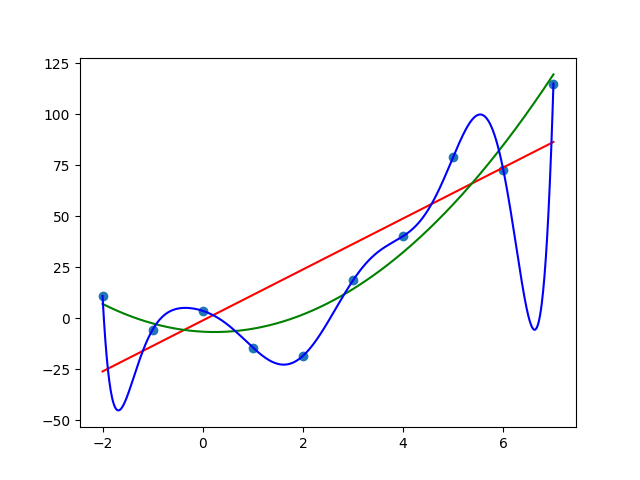
\includegraphics[width=0.6\textwidth]{overfitting.png}
\end{frame}

% --- 14. Предобработка и признаки ---
\begin{frame}{Признаки и предобработка}
	\begin{columns}
		\column{0.56\textwidth}
		\begin{itemize}
			\item Очистка: пропуски, выбросы, опечатки.
			\item Кодирование категорий, нормализация чисел.
			\item Feature engineering: новые информативные признаки.
		\end{itemize}
		\column{0.44\textwidth}
		\begin{tikzpicture}
			\node[block,fill=blue!8] (raw) {Дата: 2025-09-05};
			\node[block,fill=blue!12,below=0.5cm of raw] (feat) {День недели, месяц, выходной?};
			\node[block,fill=green!10,below=0.5cm of feat] (model) {Модель};
			\draw[arrow] (raw) -- (feat);
			\draw[arrow] (feat) -- (model);
		\end{tikzpicture}
	\end{columns}
\end{frame}
\begin{frame}{k-Nearest Neighbors (k-NN): идея}
	\textbf{Регрессия.}
	\begin{columns}[T,onlytextwidth]
		\column{0.48\textwidth}
		\textit{Одинаковые веса:}
		\[
			\hat y = \frac{1}{k} \sum_{i\in N_k(x)} y_i \, .
		\]
		\column{0.52\textwidth}
		\textit{Веса по расстоянию:}
		\[
			\hat y = \frac{\sum_{i\in N_k(x)} w_i\, y_i}{\sum_{i\in N_k(x)} w_i} \, .
		\]
	\end{columns}
	\footnotesize Замечание: метрика $d$ обычно евклидова после масштабирования признаков; $k$ и параметры весов ($p$, $h$, $\varepsilon$) подбираются по кросс-валидации.
\end{frame}


\begin{frame}{k-NN: как понимать веса (физическая интерпретация)}
	\small
	\begin{columns}[T]
		\column{0.52\textwidth}
		\textbf{Одинаковые веса (uniform).} Все соседи внутри «окна» влияют одинаково — как равномерно идущий дождь в радиусе $r$: каждая капля даёт одинаковый вклад. Это соответствует «top-hat» ядру (равномерному по диску).
		\begin{tikzpicture}
			\begin{axis}[
					width=\linewidth,height=4.8cm, xmin=0,xmax=6,ymin=0,ymax=6,
					axis lines=left, ticks=none
				]
				\addplot[only marks,mark=o] coordinates{(1.2,1.0)(1.0,1.8)(2.0,1.2)(1.6,2.1)(2.1,2.4)};
				\addplot[only marks,mark=x] coordinates{(4.2,4.7)(4.9,4.2)(3.8,4.1)(4.6,3.6)(5.1,4.9)};
				\addplot[only marks,mark=*,mark size=2.5pt] coordinates{(3.0,2.8)};
				\addplot+[domain=0:360,samples=181] ({3.0+1.4*cos(x)},{2.8+1.4*sin(x)});
			\end{axis}
		\end{tikzpicture}
		\column{0.48\textwidth}
		\textbf{Веса по расстоянию.} Ближние «тянут» сильнее, дальние — слабее: как интенсивность света или гравитация (\(\propto 1/r^2\)). Пример: $w_i=1/(d_i+\varepsilon)^p$ (обычно $p\in[1,2]$) или гауссово ядро.
		\begin{tikzpicture}
			\begin{axis}[
					width=\linewidth,height=4.8cm, xmin=0,xmax=6,ymin=0,ymax=6,
					axis lines=left, ticks=none
				]
				\addplot[only marks,mark=o] coordinates{(1.2,1.0)(1.0,1.8)(2.0,1.2)(1.6,2.1)(2.1,2.4)};
				\addplot[only marks,mark=x] coordinates{(4.2,4.7)(4.9,4.2)(3.8,4.1)(4.6,3.6)(5.1,4.9)};
				\addplot[only marks,mark=*,mark size=2.5pt] coordinates{(3.0,2.8)};
				% Визуализация "силы" влияния — линии разной толщины
				\addplot[thick] coordinates{(3.0,2.8) (2.1,2.4)}; % близко — толще
				\addplot[semithick] coordinates{(3.0,2.8) (1.6,2.1)};
				\addplot[thin] coordinates{(3.0,2.8) (1.0,1.8)};
				\addplot[thin] coordinates{(3.0,2.8) (4.6,3.6)};
				\addplot[very thin] coordinates{(3.0,2.8) (5.1,4.9)}; % далеко — тоньше
			\end{axis}
		\end{tikzpicture}
	\end{columns}
	\vspace{2pt}
	\footnotesize Выбор $k$ и типа весов — гиперпараметры: подбираются по кросс-валидации; масштабируйте признаки перед поиском соседей.
\end{frame}
\end{document}
